% !TEX program = xelatex

\documentclass[xcolor=dvipsnames, xetex,serif]{beamer}
%\documentclass[handout,xetex,serif]{beamer} %ใช้บรรทัดนี้สำหรับปริ้นเอกสาร
\usepackage{color,amsmath,graphics,graphicx}
\usepackage{epsfig,amsfonts,graphics}
\usepackage{mathrsfs,hyperref}
\usepackage{subcaption,float,framed,algorithm2e,hyperref}
%===============================================
\usepackage{fontspec,xltxtra,xunicode}
\defaultfontfeatures{Scale=1.23}
\XeTeXlinebreaklocale “th_TH” % สำหรับตัดคำ
\setmainfont[Scale=1.23]{THSarabunNew}
% 1.23 เท่าคือจาก 12 pt บน LaTeX ให้เท่ากับ 16pt บน Word
%=====================================================
%\usepackage{pgfpages} %ใช้บรรทัดนี้สำหรับปริ้นเอกสาร
%\pgfpagesuselayout{4 on 1}[a4paper,border shrink=5mm,landscape]
%\pgfpagesuselayout{2 on 1}[a4paper,border shrink=5mm]
 %ใช้บรรทัดนี้สำหรับปริ้นเอกสาร

%%%%%%%%%%%%%%% THEOREM Environments %%%%%%%%%% 					
\newtheorem{conjecture}[theorem]{บทคาดการณ์}								
\newtheorem{remark}[theorem]{หมายเหตุ}										
\numberwithin{equation}{section}							
\renewcommand\tablename{ตารางที่}
\renewcommand\figurename{รูปที่}						
\renewcommand{\bibname}{บรรณานุกรม}						
\renewcommand{\indexname}{ดรรชนี}
\setbeamertemplate{caption}[numbered]	
\setbeamertemplate{theorems}[numbered]				
%%%%%%%%%%%%%%%%%%%%%%%%%%%%%%%%%%%%%%%%%%%%%%%

\mode<presentation>{
	\usetheme{Madrid}
	\usecolortheme[named=PineGreen]{structure}}
 \title[วิธีเชิงตัวเลขสำหรับต่อเติมภาพ]{\normalsize{ขั้นตอนวิธีเชิงตัวเลขชนิดใหม่สำหรับการต่อเติมภาพที่ใช้การแปรผันรวมกับการประยุกต์สำหรับซ่อมแซมภาพจิตรกรรมไทยโบราณและการลบบทบรรยายจากอนิเมะ\\A new numerical algorithm for TV-based image inpainting with its applications for restoring ancient Thai painting images and removing subtitles from animes}}
 \author[ภัคพล]{ภัคพล พงษ์ทวี}
 \institute[SU]{
 	ภาควิชาคณิตศาสตร์\\
 	มหาวิทยาลัยศิลปากร \\}
 \date[Project Progression]{การนำเสนอความก้าวหน้าโครงงานวิจัย ครั้งที่ 2\\
 	9 เมษายน 2562}
 
 \AtBeginSubsection[]{
 	\begin{frame}<beamer>
 		\frametitle{Outlines}
 		\tableofcontents [currentsection,currentsubsection]
 	\end{frame}}
 	%\setbeamertemplate{item}[square]
 	%============================================================================
 	\begin{document}
 		\begin{frame}
 			\titlepage 
		 \end{frame}
		 \begin{frame}
			\frametitle{ความคืบหน้า}
			\centering
			\begin{figure}
				\begin{subfigure}{0.4\linewidth}
					\centering
					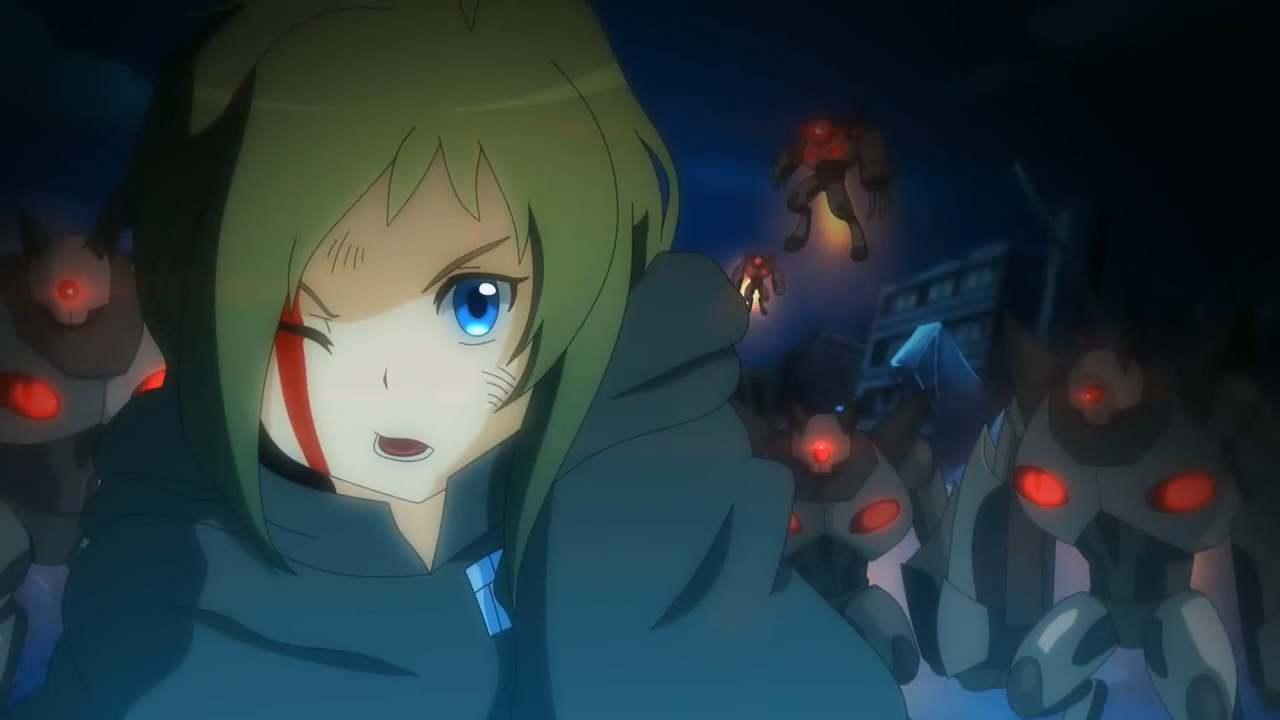
\includegraphics[width=0.8\linewidth]{images/inori-preview.png}
					\caption*{{\large การลบคำบรรยายอนิเมะ}}
				\end{subfigure}
				\begin{subfigure}{0.4\linewidth}
					\centering
					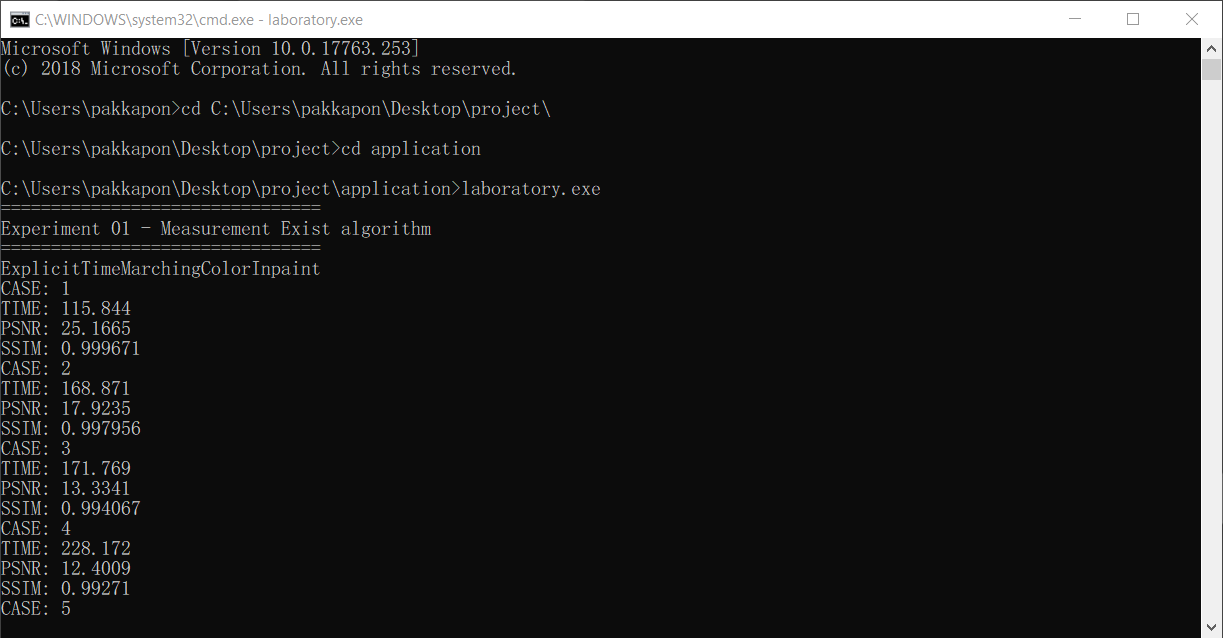
\includegraphics[width=0.8\linewidth]{images/software_appendix/laboratory.png}
					\caption*{{\large โปรแกรมที่ได้พัฒนาขึ้น}}
				\end{subfigure}	
			\end{figure}
		\end{frame}
		\begin{frame}
			\frametitle{ผลการลบบทบรรยาย}
			\begin{table}[H]
				\centering
				\captionsetup{justification=centering}
				\begin{tabular}[ht]{|l|c|c|c|c|}
					\hline
					วิธีการ  & เวลาประมวล  (วินาที) & PSNR (dB) & SSIM \\
					\hline
					สปริทเบรกแมน & * & * & * \\
					วิธีการที่พัฒนาขึ้น & 75.76 & 29.33 & 0.9454 \\
					\hline
				\end{tabular}
				\caption{ผลการลบบทบรรยายออกจากอนิเมะเฉลี่ย\\โดยวิธีการสปริทเบรกแมนและวิธีการที่พัฒนาขึ้น}
			\end{table}	
		\end{frame}
		\begin{frame}
			\frametitle{ผลการลบบทบรรยาย (ต่อ)}
			\begin{table}[H]
				\centering
				\captionsetup{justification=centering}
				\begin{tabular}[ht]{|l|c|c|c|c|}
					\hline
					วิธีการ  & เวลาประมวล  (วินาที) & PSNR (dB) & SSIM \\
					\hline
					สปริทเบรกแมน & 5,073.08 & 32.88 & 0.9654 \\
					วิธีการที่พัฒนาขึ้น & 75.76 & 29.33 & 0.9454 \\
					\hline
				\end{tabular}
				\caption{ผลการลบบทบรรยายออกจากอนิเมะเฉลี่ย\\โดยวิธีการสปริทเบรกแมนและวิธีการที่พัฒนาขึ้น (ต่อ)}
			\end{table}	
		\end{frame}
		\begin{frame}
			\frametitle{โปรแกรมทดสอบการซ่อมแซมภาพศิลปะไทย}
			\begin{figure}
				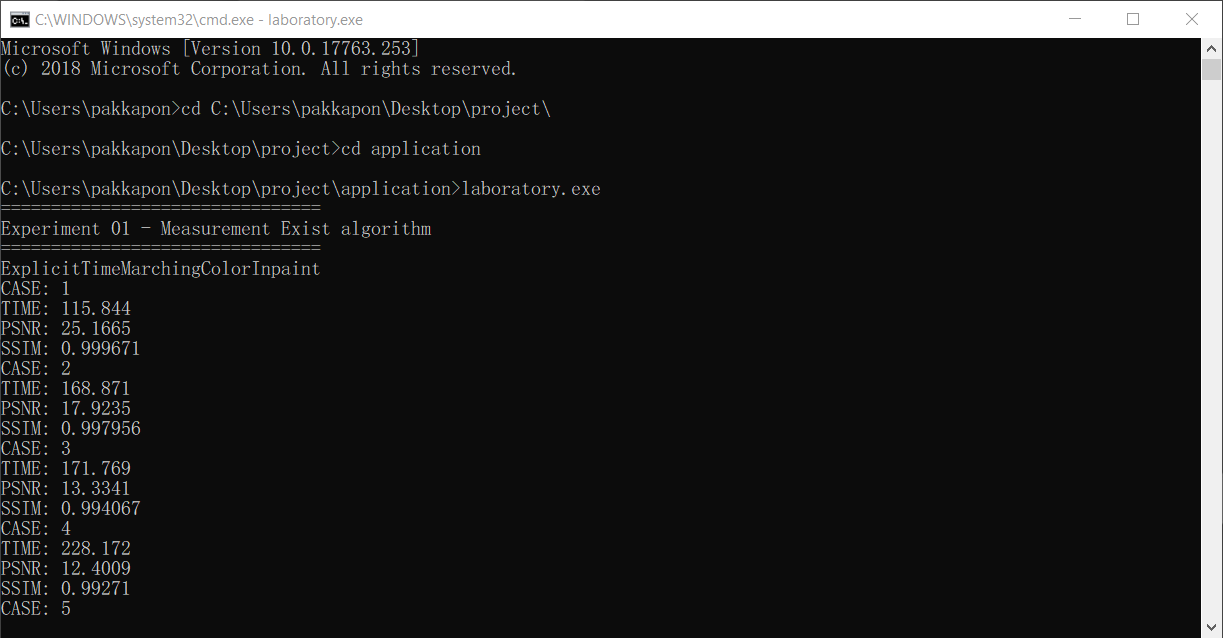
\includegraphics[width=0.8\linewidth]{images/software_appendix/laboratory.png}
				\caption{โปรแกรมทดสอบการซ่อมแซมภาพศิลปะไทย}
			\end{figure}
		\end{frame}
		\begin{frame}
			\frametitle{โปรแกรมทดสอบการลบคำบรรยาย}
			\begin{figure}
				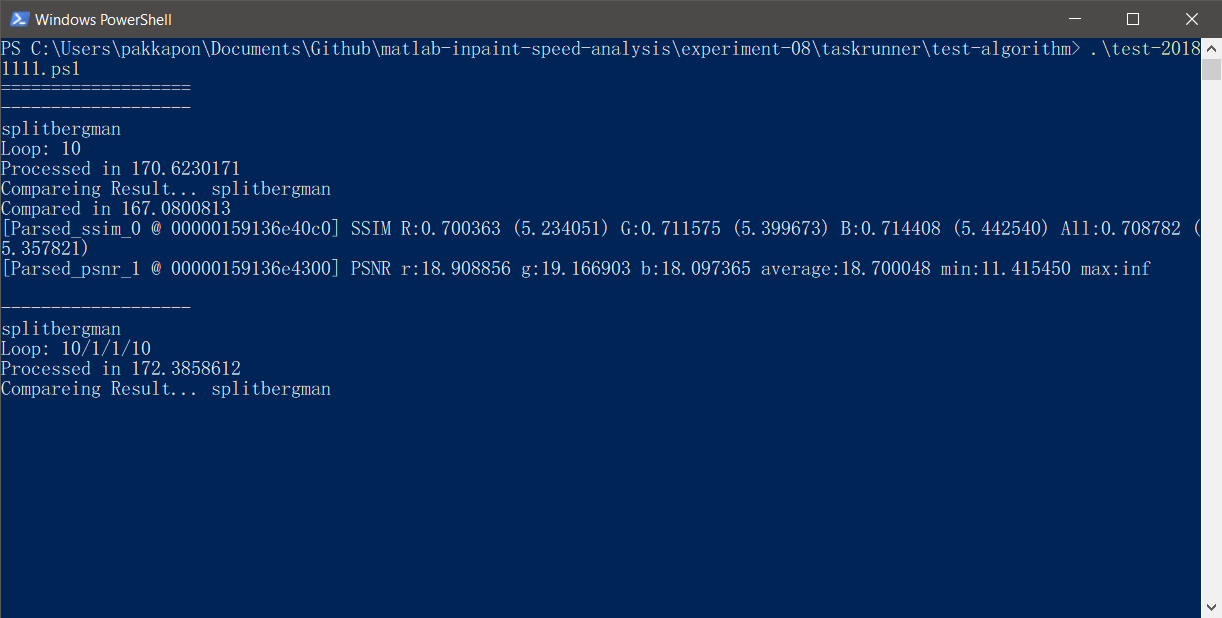
\includegraphics[width=0.8\linewidth]{images/software_appendix/lab_remove.png}
				\caption{โปรแกรมทดสอบการลบคำบรรยาย}
			\end{figure}
		\end{frame}
		\begin{frame}
			\frametitle{โปรแกรมทดสอบการซ่อมแซมภาพศิลปะไทย บน Colab}
			\begin{figure}
				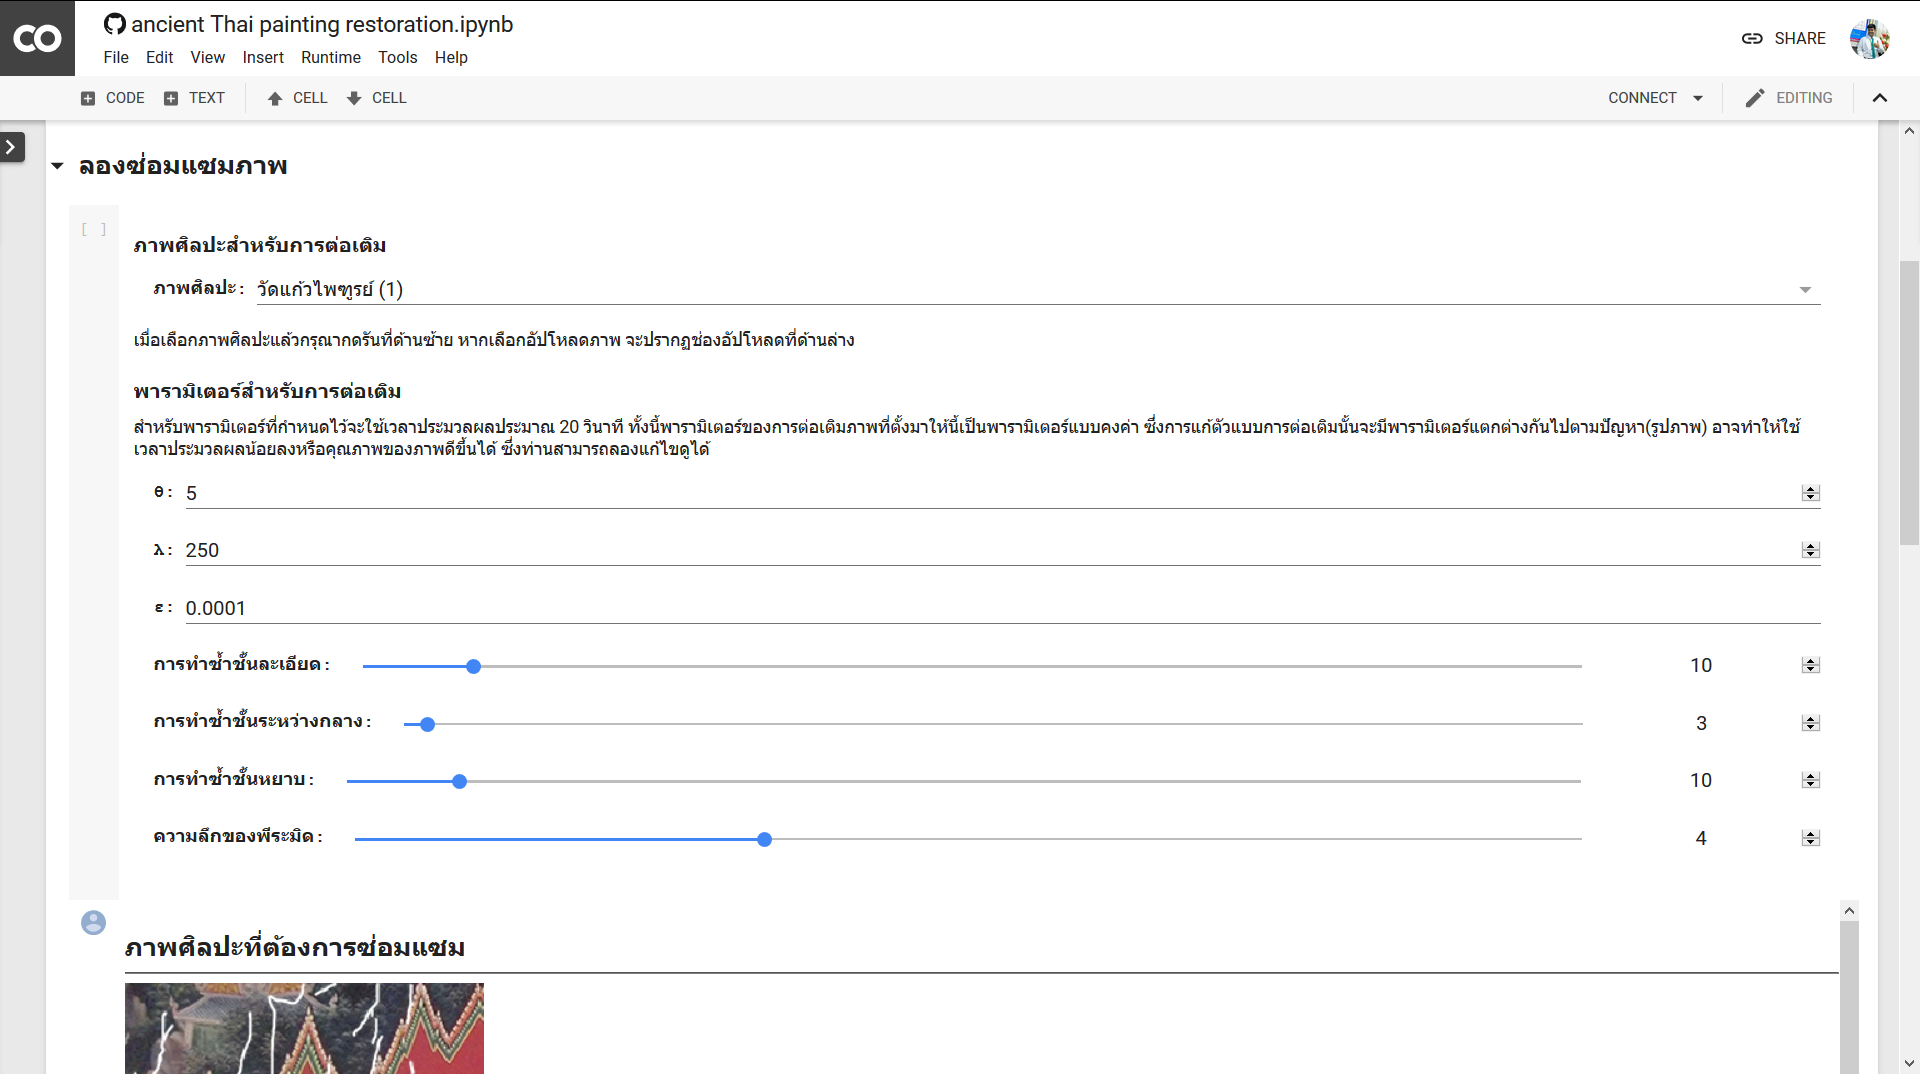
\includegraphics[width=0.8\linewidth]{images/colab/colab_preview.png}
				\caption{โปรแกรมซ่อมแซมภาพศิลปะไทยบน Colab (bit.ly/demothai)}
			\end{figure}
		\end{frame}
		\begin{frame}
			\frametitle{โปรแกรมทดสอบการซ่อมแซมภาพศิลปะไทย บน Colab (ต่อ)}
			\begin{figure}
				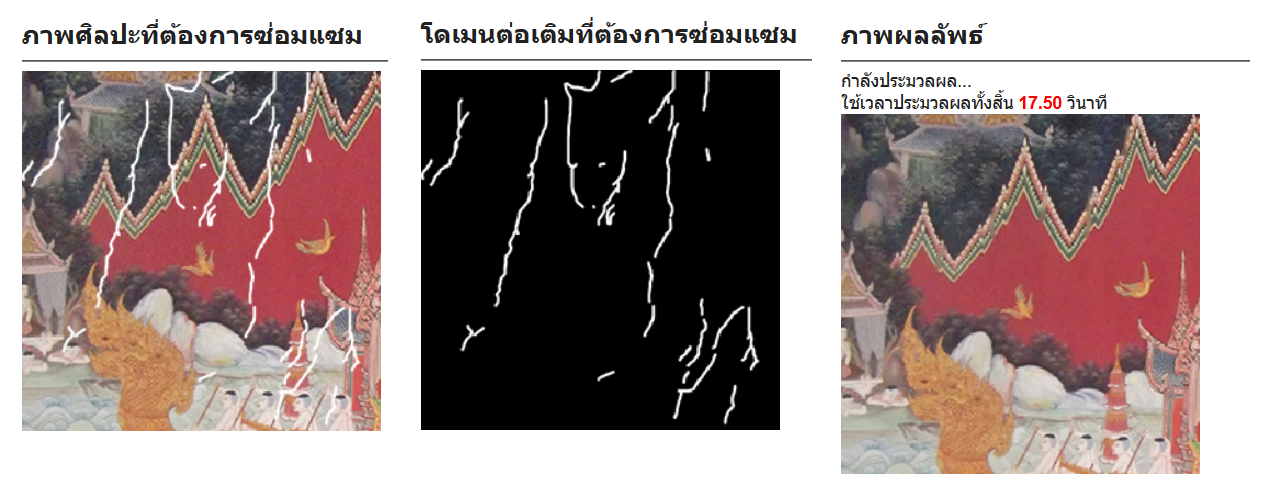
\includegraphics[width=0.8\linewidth]{images/colab/inpaint_display.png}
				\caption{ตัวอย่างผลลัพธ์การซ่อมแซมภาพศิลปะไทย}
			\end{figure}
		\end{frame}
		\begin{frame}
			\frametitle{โปรแกรมลบคำบรรยาย}
			\begin{figure}
				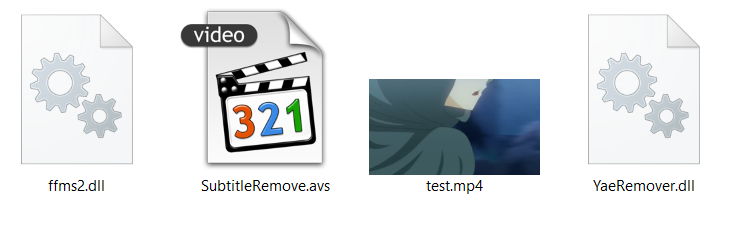
\includegraphics[width=0.8\linewidth]{images/demo_anime/file.png}
				\caption{ชุดไฟล์สำหรับลบคำบรรยาย (bit.ly/demo-anime-inpaint)}
			\end{figure}
		\end{frame}
		\begin{frame}
			\frametitle{โปรแกรมลบคำบรรยาย (ต่อ)}
			\begin{figure}
				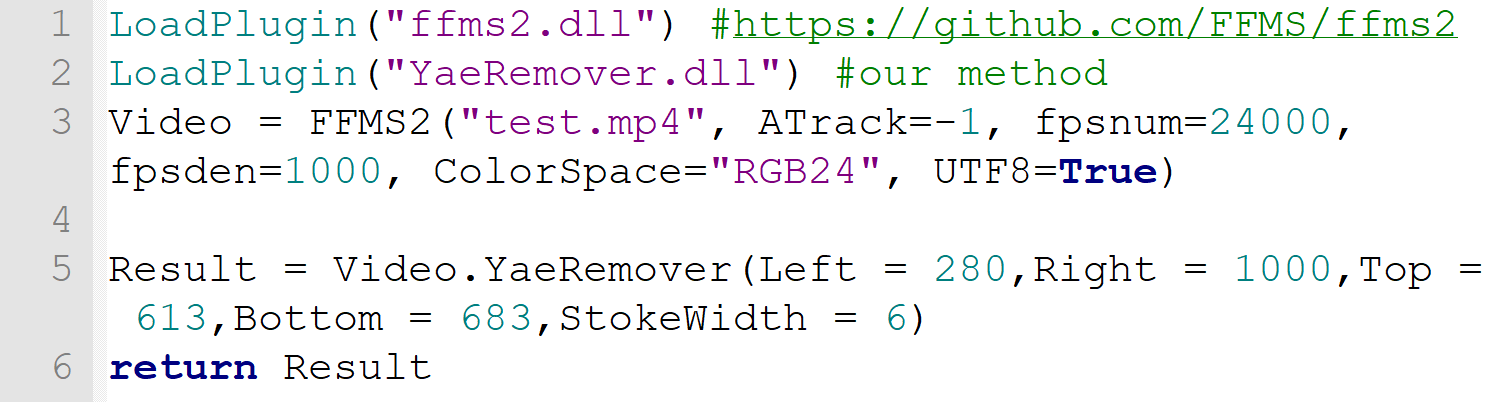
\includegraphics[width=0.8\linewidth]{images/demo_anime/notepad.png}
				\caption{โค้ดภายใน SubtitleRemove.avs}
			\end{figure}
		\end{frame}
		\begin{frame}
			\frametitle{โปรแกรมลบคำบรรยาย (ต่อ)}
			\begin{figure}
				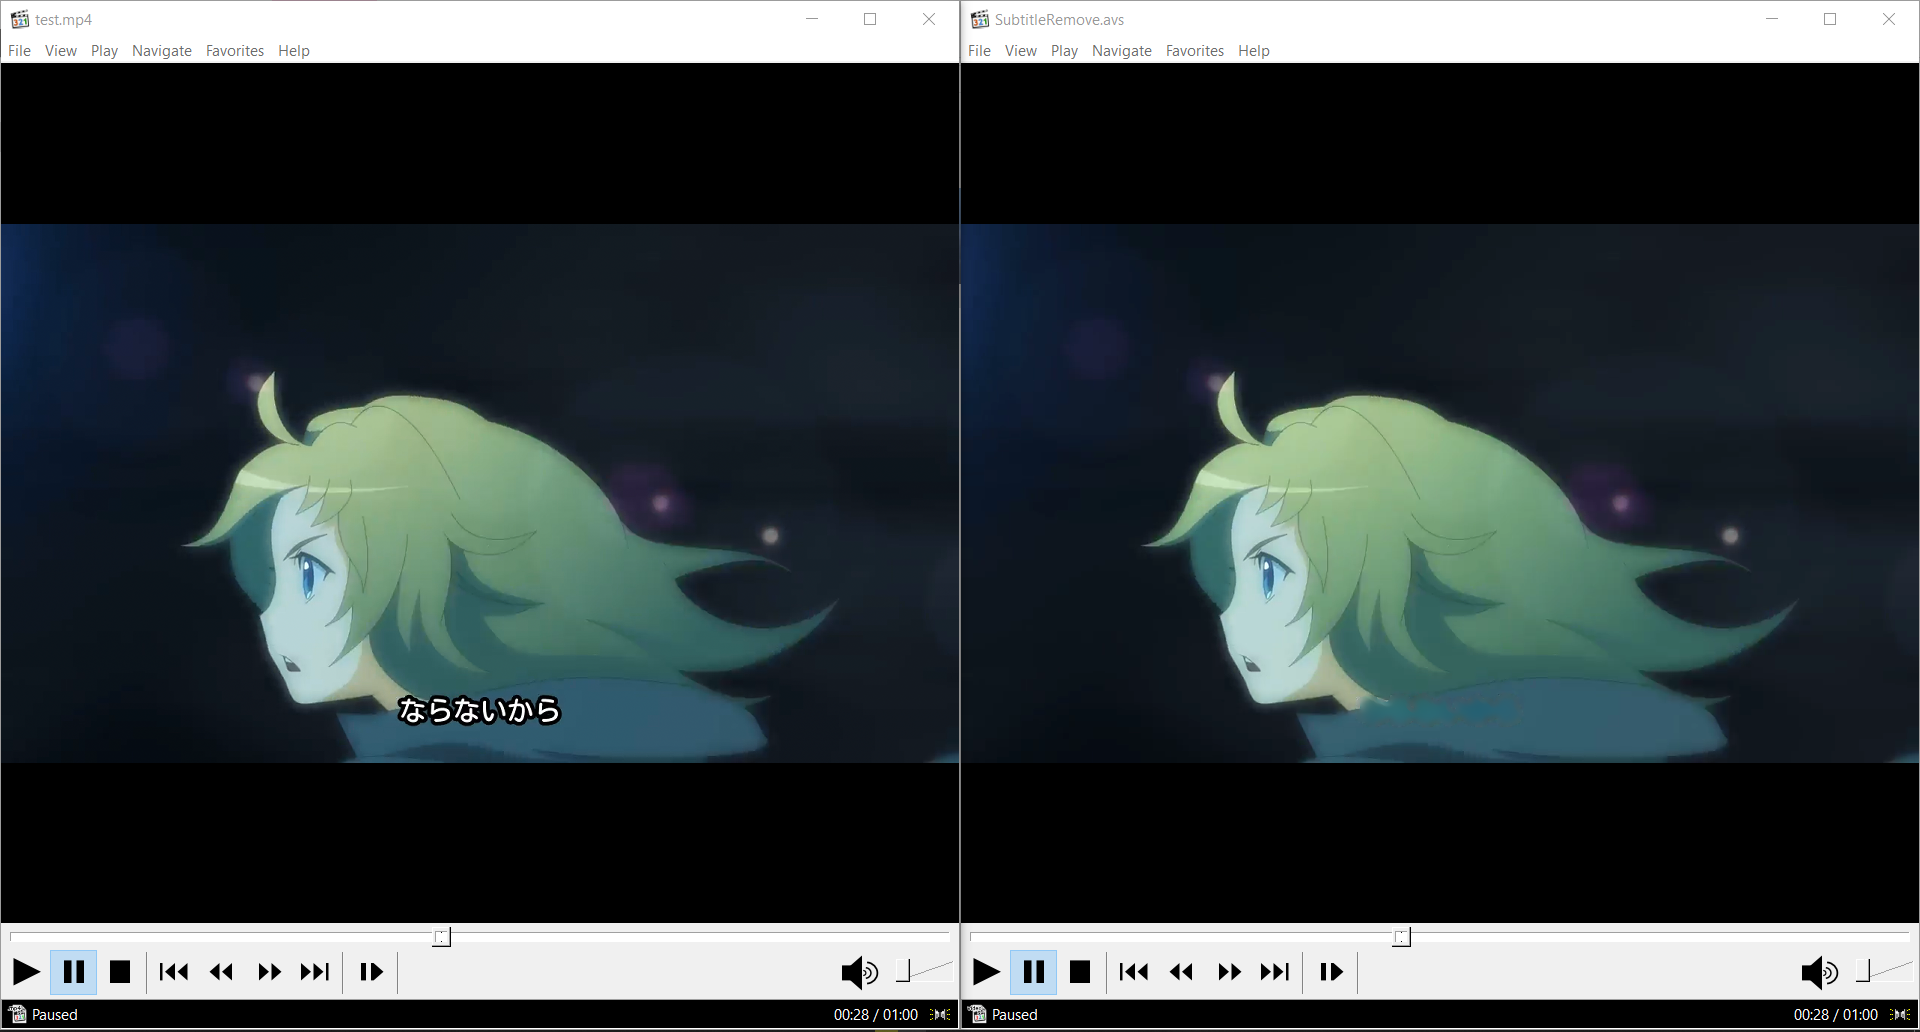
\includegraphics[width=0.8\linewidth]{images/demo_anime/result.png}
				\caption{test.mp4 (ซ้าย) และ SubtitleRemove.avs (ขวา) เมื่อเปิดด้วย MPC-HC}
			\end{figure}
		\end{frame}
		\begin{frame}
			\centering
			\Huge{ขอขอบคุณ}
		\end{frame}
	\end{document}





